\chapter{Introduction}
\label{chapter:intro}
\graphicspath{{./chapters/c1_intro/figures/}}
%=========== MAIN ================
This chapter contains the basics needed for the work done in this thesis.
Towards the end of this chapter, an overview of all the chapters is given.
%============== MAIN ================
\section{Fluorescence}
The absorption and subsequent emission of light by materials is called fluorescence.
The term Fluorescence was named by \textit{George Gabriel Stokes} after observing ultraviolet light being transformed into visible light in the mineral fluorite.\cite{Stokes1852}
A molecule is excited to a higher electronic energy state after absorbing a resonant photon.
Each electronic energy level is associated with vibrational and rotational energy levels.
The excess vibrational energy gained in the excited state is quickly lost to the surrounding in a time period of sub-picoseconds and the molecule stay in its zero vibrational level of excited state for about nanoseconds..
If it allowed to come down to the ground state which is decided by the spin states (singlet allowed) of the paired the electrons and Franck-Condon principle, \textit{fluorescence emission} is observed.
The emitted photon has a smaller energy than the absorbed photon leading to Stoke's shift and the total time it takes to come down to the ground state is called fluorescence lifetime typically \SI{10}{\ns}.
If the system crosses over from singlet excited to the triplet state, emission may be observed at even longer wavelength and even longer lifetime which is known as \textit{phosphorescence}.
The processes between the absorption and the emission is normally represented graphically by Jablonski diagram.
\begin{figure}
	\centering
	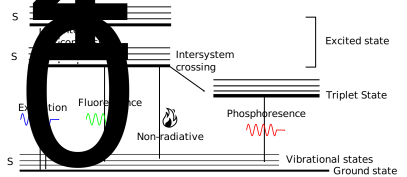
\includegraphics[width=0.8\textwidth]{jablonski}
	\caption{\textbf{Jablonski Diagram}}
	\label{fig:jablonski}
\end{figure}

Natural materials that show fluorescence include minerals, tissue in plants and animals.
Among biological molecules nicotinamide adenine dinucleotide (NADH), flavins (FAD), chlorophyll are abundantly found fluorescing.
Extrinsic fluorophores are also synthesized with high quantum yield and varying color which include synthetic dyes, quantum dots.
Fluorescence has a huge advantage of very low background which enables their detection with very low concentration of fluorescent molecules.
This was very important for biological imaging as little quantity of such markers keep the system under study unaffected.
Not only external fluorophores can be used for biological marking, the cells can also be gene-edited to produce their own fluorophores called fluorescent protein (GFP).
Now a days it is unthinkable to use a biology or analytical chemistry lab without fluorescence technique.

\section{Single Molecule Spectroscopy}
The thought experiment by Jean Perrin to observe single fluorescent molecules was materialized for the first time in 1990s at extremely low temperature and in an advanced laboratory.\cite{orrit1990single}
The rapid development of optical microscope, lasers, dyes and detectors now made it possible to detect single molecules at room temperature on a bench top.\cite{xie1998optical,weiss1999fluorescence,moerner1999illuminating}
Not only it has grown itself into an important research field, the concept is now heavily used in molecular biology, super-resolution microscopy, quantum computing, catalysis to name a few.\cite{zhuang2000a,huang2008threedimensional,eisaman2011invited,lounis2005singlephoton,roeffaers2007singlemolecule}
The following advantages provided by single-molecule study makes it an indispensable technique:
\begin{itemize}
	\item \textbf{No averaging.} Ensemble measurements provide mean value of a physical quantity, looking at average behavior of vast number of molecules.
	In complex medium like in condensed matters and cellular matrix, each molecule is in a different microscopic surrounding experiencing different forces and resistances.
	Single molecule measurements provide distribution of quantities distinguishing the subpopulations within the system with similar characteristics.
	For example different host molecules even in a crystalline (ordered structure) solids shows different spectral lines and line widths discovering the imperfections.\cite{kozankiewicz1994single,reilly1993spectral}
	Small domains of \SIrange{50}{700}{\nm} in a cell membrane are located based on the difference in their diffusion coefficient.\cite{lommerse2004singlemolecule}
	Rare species that are lost in ensemble measurements can be identified and investigated in SM studies.
	The distribution in spatial dimension is called static heterogeneity.
	\item \textbf{Time dependent fluctuation.} Dynamics of systems can be studied without the need for synchronization (kinetic measurements in ensemble often require synchronization).
	Single molecule measurements at equilibrium provide direct access to both dynamics and statistics of molecular complexes.
	They also provide information on a wide range of time scale from microseconds to tens of seconds extracting translational, orientational, enzymatic-turnovers and protein folding-unfolding events.
	\item \textbf{Local reporter} As single molecule detection is based on optical microscopy, the observer can be far away from the molecule itself provided the intervening medium is optically transparent.
	The trajectory of the reporter molecules deep inside the cell can be tracked to follow the activities of the host.
	\item \textbf{Tool.} Single-molecules are finding their ways to be used tools to perform different tasks.
	As the transitions in the excitation of single-molecules are quantum in nature, they can be used as pure source of single photons for quantum computing.
	The single step blinking nature of single molecules has been used for super localization and there by spatially differentiating up to nanometer scale.
	Moerner, Betzig and Hell were awarded Nobel prize in Chemistry in 2014 for their contribution towards super-resolution microscopy and single-molecule detection.
\end{itemize}
Here we discussed some of the applications of Single-molecule measurements which provide plethora of information and the possibilities are only limited by the practitioner's creativity and imagination.

Two major characteristics that proves the detection of Single molecules are their stepwise changes of intensity and anti bunching.
Molecules in their excited state can cross over to triplet state resulting in loss of emission until the molecules comes back to the ground state to keep the excitation-emission cycle going.
This results in blinking of intensity between two levels.
A molecule on the triplet state is more reactive because of its unpaired electrons and can react with triplet oxygen in the system leading to bleaching and complete loss of fluorescence.
Both one step blinking and bleaching information can be used to identify single molecules.
Single molecules are quantum systems that can only emit one photon at a time.
When the photon stream from the molecule is sent to two detectors via a beam splitter, anti bunching is observed in the autocorrelation of the two spitted signals.
Such anti bunching experiments to determine the singleness of the photon source is known as ``Hanbury-Brown Twiss  measurement''.
\begin{figure}
	\centering
	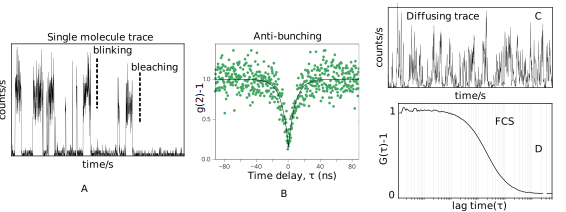
\includegraphics[width=\textwidth]{SM_characteristics}
	\caption{\textbf{Single-molecule characteristics.}
	(A) Time trace of a single molecule showing single-step switching (blinking) and bleaching.
	Notice the reappearance of the intensity after blinking but complete disappearance after bleaching.
	(B) Anti-bunching at zero delay time in the correlation shows the singleness of the emitter.\cite{chu2016a}
	(C) Time trace of diffusing molecules in a fluid with \SI{1}{\nM} fluorophores showing intensity bursts and the correlation amplitude ($G(\tau)-1={\sim}1$) indicates the presence of few molecules in the focus.}
	\label{fig:SM_characteristics}
\end{figure}

Fluorescence correlation spectroscopy (FCS) also considered as a single-molecule technique, measures the temporal correlation of fluctuating light intensities.
Conventional way to perform FCS is to collect signal from \textit{diffusing fluorescent} molecules in the diffraction limited focal volume and then compute the autocorrelation of the intensity trajectory.
The autocorrelation of the intensity signal is given as $G(\tau)=<I(t)I(t+\tau)>/<I(t)>^2$ where I is the intensity, $\tau$ the lag time and $<...>$ represents time averaging.
The correlation quantifies the probability the intensity at time $t$ is similar to the intensity at a later time $t+\tau$.
It provides information on the concentration and the time scale of the fluctuating observable.
By very nature, FCS technique require the fluctuation of the number of diffusing fluorophores in the diffraction limited volume of \SI{1}{fL}, ideally one molecule in average which translates to a concentration of \SI{1}{\nM}.
Because of the diffraction limit ($\Delta{x}={\lambda}/2$), FCS is often limited to nanomolar concentration of the analyte. 

Two of the important requirements to measure single molecules with high spatial and temporal resolution are (i) high fluorescence yield and (i) small excitation and detection volume.
In this thesis we push the limit of single-molecule detection to low quantum yield dyes and to high concentration of fluorophore.
\section{TCSPC}

\section{FRET}
%
\section{Optical Nanoantennas}
\section{Gold nanorod surface plasmon}
\section{Fluorescence Enhancement by plasmonics}
%
\section{Enzymology and Electron transfer}
\section{Protein at work are Proteins in Motion}
\section{Azurin: a copper containing redox protein}
\section{Flurox Principle}
\subsection*{FRET as Redox state indicator}
%
\section{This thesis}
